
\chapter{\'Etude du corpus de son \textit{grafic}}
\label{chap:grafic}

Au chapitre précédent, le comportement de la NMF vis à vis des environnements sonores urbains a été étudiée avec l'aide du corpus élémentaire \textit{Ambiance}. Ce corpus était composé d'une composante \textit{trafic} dont le niveau sonore était calibré avec des sources sonores spécifiques isolées. Si cette partie a permis de démontrer l'intérêt de la NMF IS sur de tels environnements sonores, les performances et les combinaisons obtenus ne correspondent toutefois pas à celles qui seraient adaptées à des enregistrements sonores. Ainsi, dans ce chapitre, la NMF est appliquée sur un corpus d'évaluation \textit{SOUR}, composé de scènes sonores simulées et dont le réalisme a été validé par le test perceptif présenté en chapitre \ref{sec:test}. Ce réalisme permet de s'assurer que les scènes du corpus sont assimilables à des enregistrements sonores et donc de la validité des résultats émis par la NMF. L'approche qui obtient les erreurs les plus faibles pourra alors être intégré dans des capteurs embarqués pour estimer le niveau sonore du trafic routier. Dans un premier temps, un rappel du corpus, des facteurs expérimentaux, de leur modalités respectifs et de la métrique employée sont rappelés. Puis les erreurs générés par l'estimateur \textit{baseline} et par la NMF sont présentés. Des pistes visant à améliorer ces estimations sont ensuite étudiées et proposées.

\section{Rappel des facteurs expérimentaux}
 

\begin{figure}[hbtp]
\centering
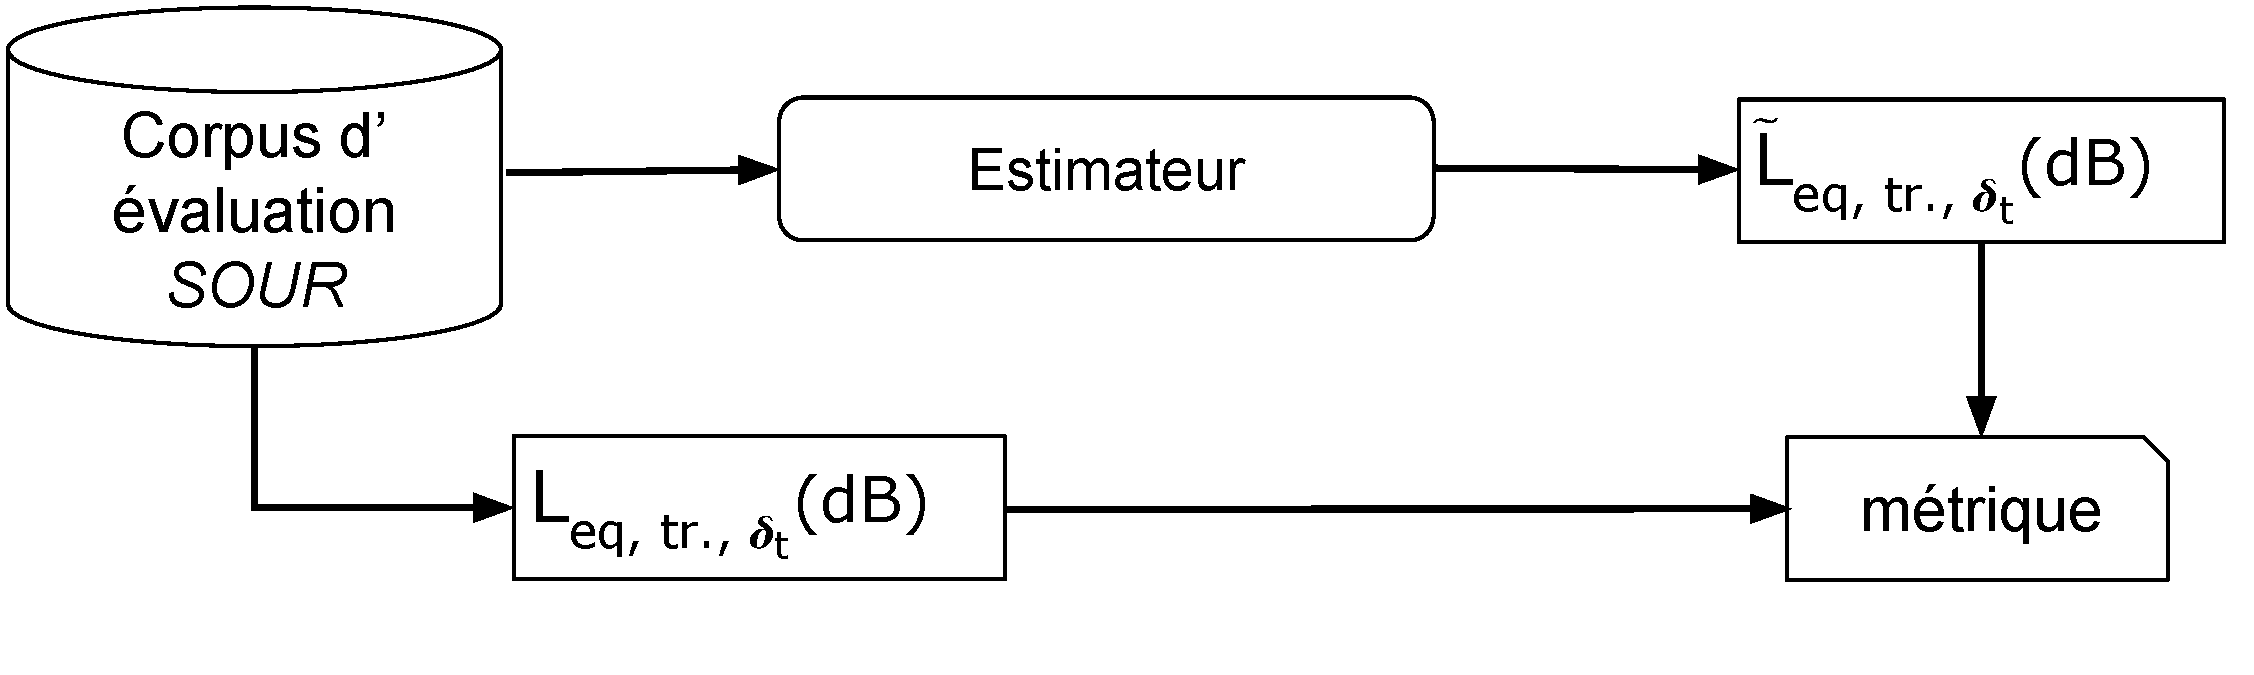
\includegraphics[width=0.9\linewidth]{./figures/NMF/Bloc_diagram_estimateur_SOUR.pdf}
\caption{Diagramme en blocs des étapes dans l'estimation du niveau sonore du trafic.}
\label{fig:diagram_SOUR}
\end{figure}


De prime abord, les étapes mis en place dans cette partie sont similaires à celles du chapitre précédent et sont présentées dans la Figure \ref{fig:diagram_SOUR} : les scènes sonores du corpus d'évaluation \textit{SOUR} sont soumis à un estimateur qui détermine le niveau sonore du trafic estimé, $\tilde{L}_{eq,tr.}$ qui est comparé à sa valeur exacte, $L_{eq,tr.}$ par le calcul d'une métrique.
Le corpus d'évaluation \textit{SOUR}, présenté en détail dans la partie \ref{part:corpus_grafic}, est composé de 74 fichiers audio d'une durée totale de 2h50, divisé en 4 ambiances sonores : \textit{Parc} (8 scènes, abrégé \textit{Pa.}), \textit{Rue calme} (35 scènes, abrégé \textit{Ca.}), \textit{Rue bruyante} (23 scènes, abrégé \textit{Br.}), \textit{Rue très bruyante} (8 scènes, abrégé \textit{Tr. Br.}). Ce corpus a été réalisé à partir d'enregistrements sonores et de leur annotations afin d'obtenir une structure temporelle de ces scènes simulées similaires à des enregistrements sonores. La qualité et le réalisme de ces scènes a été validée auprès d'un test perceptif. Assimilable à des enregistrements sonores, ces scènes permettent de simuler les comportements de la NMF face à des scènes similaires à des enregistrements sonores réalisés en ville. Comparé au corpus \textit{Ambiance}, ces scènes présentent une part du trafic plus importante et mélange des sources sonores multiples (aboiement de chien, sifflement d'oiseaux, voix, bruit de rue, bruit de pas, sonnerie, portes).

Chaque scène est alors soumise à un estimateur qui permet l'estimation du niveau sonore du trafic routier. 
Le premier estimateur \textit{baseline} reste le même que dans le chapitre \ref{chap:ambiance} : un filtre passe-bas de fréquence de coupure $f_c$ avec $f_c \in \lbrace 100,~500,~1k,~2k,~5k,~10k,~20k \rbrace$ Hz. L'application reste similaire que dans le chapitre précédent (voir Figure \ref{fig:baseline}) : le spectrogramme du signal audio est coupé à la fréquence $f_c$ et toute l'énergie située dans la bande passante est assimilée au trafic routier.
Le second estimateur est basé sur la NMF où l'on considère l'apprentissage supervisée (NMF SUP), semi-supervisée (NMF SEM) ainsi que la NMF seuillée initialisée (NMF IS). Le choix de la $\beta$-divergence reste circonscrit à $\beta \in \lbrace 0,~1,~2 \rbrace$.
L'apprentissage du dictionnaire suit les même étapes que dans le chapitre précédent : chaque spectrogramme, issus des 53 fichiers audio constituant le corpus d'apprentissage, est découpé en trame temporelle de durée $w_t \in \lbrace 0,5,~1,~2 \rbrace$. Les valeurs \textit{rms} sont ensuite calculées selon la fréquence. L'algorithme de clustering $K$-mean est ensuite appliquée. Comme le corpus est plus petit et que ce facteur s'est révélé influent, on étend le nombre d'éléments dans $\mathbf{W}$ à $K \in \lbrace 25,~50,~100,~200,~ 300 \rbrace$. Le cas \textit{all} où la valeur \textit{rms} est calculée sur l'intégralité du corpus est aussi conservé avec une réduction des matrices restreint à $K_{w_t = all} = \lbrace 25,~50 \rbrace$. Les dictionnaires constitués d'éléments \textit{trafic} compose le dictionnaire $\mathbf{W}$ de la NMF SUP, le dictionnaire $\mathbf{W_s}$ de la NMF SEM et le dictionnaire $\mathbf{W_0}$ de la NMF IS.
Pour la NMF SEM, le nombre d'éléments dans le dictionnaire $\mathbf{W_r}$ est maintenu à $J = 2$.
Dans le cas de la NMF IS, l'influence de l'opérateur sigmoïde dans le calcul de la distance et l'utilisation du seuil \textit{firm} s'étant relevées très faibles, l'étude se réduit au seul cas de la représentation linéaire de la distante $D_{\theta}$ avec un seuillage dur de seuil $t_h$.
Comme les scènes sonores sont plus longues (de 1 min jusqu'à 3 minutes), le nombre d'itération est étendu à 400. 
Le résumé de ces facteurs expérimentaux et de leur modalités respectives se trouve dans le Tableau \ref{tab:experimental_factorsNMF}.

\begin{table*}[t]
\centering
\caption{Facteurs expérimentaux et leur modalité utilisé pour le corpus \textit{SOUR}.}
\begin{tabularx}{17.5cm}{L{3cm}@{}C{12cm}@{}C{2cm}@{}}
	\hline
    \textbf{\begin{tabular}[c]{@{}l@{}}facteur \\ expérimentaux \end{tabular}} & \textbf{modalités} & \begin{tabular}[c]{@{}C{2cm}@{}}\textbf{nombre de}\\ \textbf{modalité}\end{tabular}\\ \toprule
\end{tabularx}

\begin{tabularx}{17.5cm}{L{3cm}@{}C{3cm}@{}@{}C{3cm}@{}@{}C{3cm}@{}@{}C{3cm}@{}C{2cm}@{}}
    \textbf{Environnement sonore} & \begin{tabular}[c]{@{}c@{}}parc\\ 'Pa'\end{tabular} & \begin{tabular}[c]{@{}c@{}}rue calme \\ 'Ca'\end{tabular} & \begin{tabular}[c]{@{}c@{}}rue bruyante\\ 'Br' \end{tabular}& \begin{tabular}[c]{@{}c@{}}rue très bruyante\\ 'TrBr'\end{tabular} & 4\\
\end{tabularx}

\begin{tabularx}{17.5cm}{L{3cm}@{}C{3cm}@{}@{}C{3cm}@{}@{}C{3cm}@{}@{}C{3cm}@{}C{2cm}@{}}
	\rowcolor[HTML]{C0C0C0}
  \textbf{méthode} & filtre passe bas & NMF SUP & NMF SEM & NMF IS & 4\\
\end{tabularx}

\begin{tabularx}{17.5cm}{L{3cm}@{}@{}C{1.714cm}@{}@{}C{1.714cm}@{}@{}C{1.714cm}@{}@{}C{1.714cm}@{}@{}C{1.714cm}@{}@{}C{1.714cm}@{}@{}C{1.714cm}@{}C{2cm}@{}}
   $\mathbf{f_c}$ (kHz) & 1 & 0.5 & 1 & 2 &  5 & 10 & 20 & 7\\
\end{tabularx}

\begin{tabularx}{17.5cm}{L{3cm}@{}C{3cm}@{}@{}C{3cm}@{}@{}C{3cm}@{}@{}C{3cm}@{}C{2cm}@{}}
\rowcolor[HTML]{C0C0C0}
    $\mathbf{w_t}$ (s)& 0.5 & 1 & 2 & \textit{all} & 4\\
\end{tabularx}

\begin{tabularx}{17.5cm}{L{3cm}@{}C{2.4cm}@{}@{}C{2.4cm}@{}@{}C{2.4cm}@{}@{}C{2.4cm}@{}@{}C{2.4cm}@{}C{2cm}@{}}
    $\mathbf{K}$ & 25 & 50 & 100 & 200 & 300 & 5\\
\end{tabularx}

\begin{tabularx}{17.5cm}{L{3cm}@{}C{4cm}@{}@{}C{4cm}@{}@{}C{4cm}@{}C{2cm}@{}}
\rowcolor[HTML]{C0C0C0}
   $\mathbf{\beta}$ & 0 & 1 & 2 & 3\\
\end{tabularx}

\begin{tabularx}{17.5cm}{L{3cm}@{}C{12cm}@{}C{2cm}@{}}
   seuillage dur $\mathbf{t_h}$ & de 0.20 à 0.60 avec un pas de 0.01 & 41\\
   \bottomrule
\end{tabularx}
\label{tab:experimental_factorsNMF}
\end{table*}

 
En sortie de l'estimateur est calculé un niveau sonore global du trafic, $\tilde{L}_{eq,tr.,\delta_t}$. Dans le précédent corpus, comme chaque scène était d'une durée similaire, les niveaux sonores équivalent étaient calculés pour une durée d'intégration $\delta_t$ de 30 secondes. Ici, la durée des scènes dans le corpus \textit{SOUR} est variable. Pour harmoniser le calcul de la métrique, c'est une erreur toute les 60 secondes qui est calculée, $MAE_{60}$ : 

\begin{equation}
MAE_{60} = \frac{\sum_{i = 1}^{N_{60}}\vert L_{eq,tr.,60s, i} - \tilde{L}_{eq,tr.,60s, i}\vert}{N_{60}}
\end{equation}

avec l'expression du niveau sonore pour la scène $i$ $L_{eq,tr.,60s, i}$,  

\begin{equation}
L_{eq,tr.,60s, i} = 10 \times \log_{10}\left(\frac{1}{60}\int_{t_{init}}^{t_{init}+60} 10^{L_{p,tr.}(t)/10} dt\right)
\end{equation}

Pour cela, les signaux \textit{trafic} obtenus en sortie de l'estimateur sont cumulée les uns à la suite des autres. Puis le niveau sonore équivalent est successivement calculé pour une durée d'intégration $\delta_t$ de 60 secondes. Il est alors possible de calculer un $MAE_{60}$ dont une partie de l'erreur est calculé sur une scène et l'autre partie sur la scène suivante. On résume en Figure \ref{fig:exempe_mae60}, un exemple du procédé. 

\begin{figure}[ht]
\centering
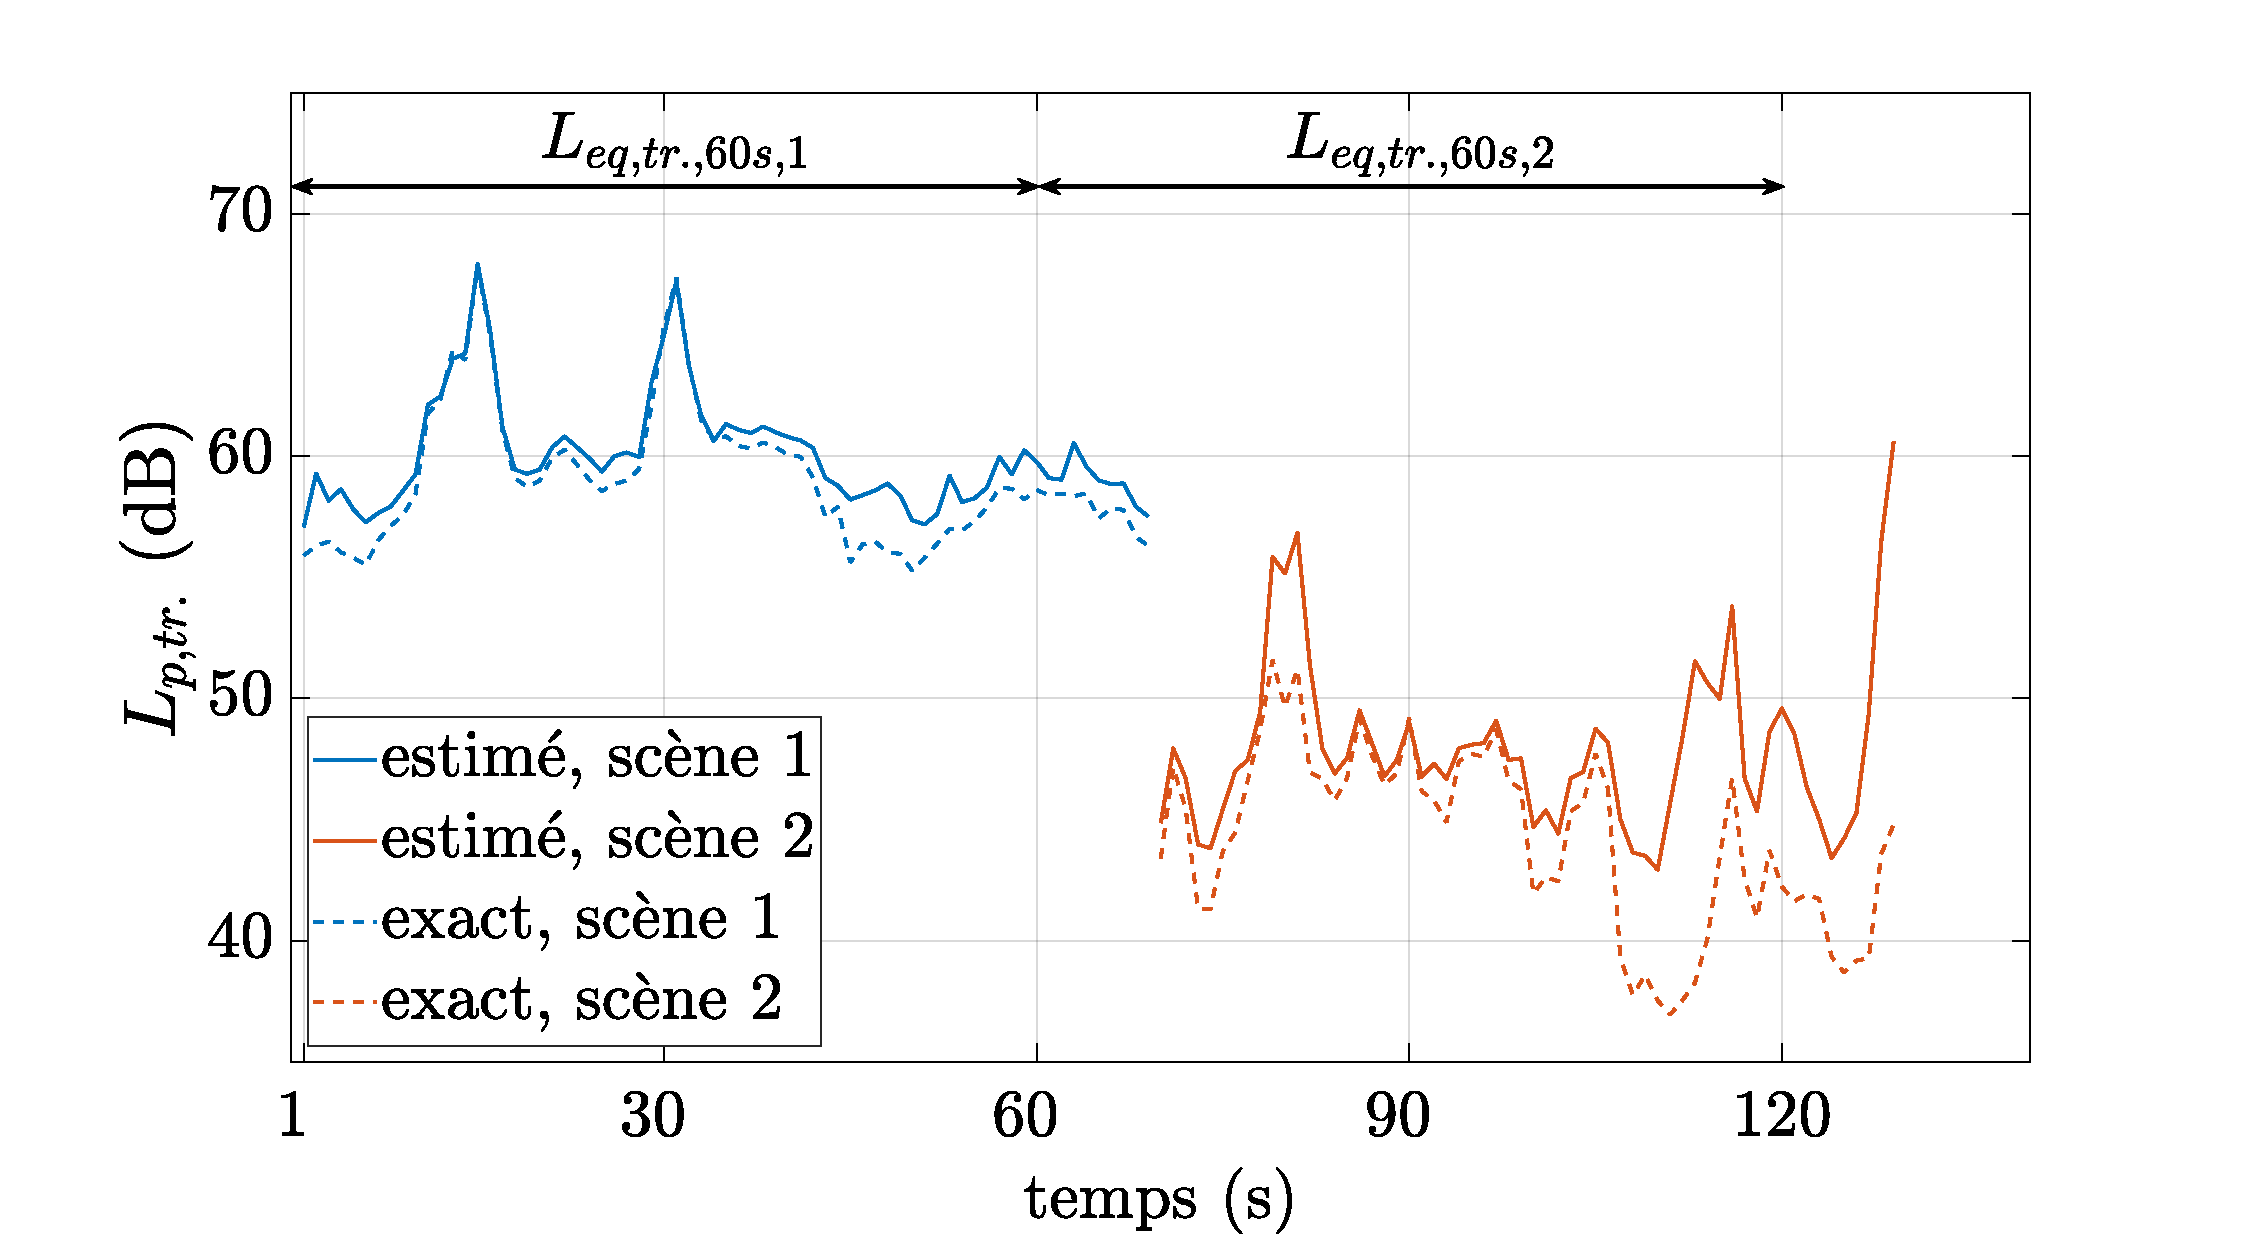
\includegraphics[width=.9\linewidth]{./figures/resultats/Lp_mae.pdf}
\caption{Estimation des niveaux sonores équivalents pour une durée d'intégration de 60 secondes sur deux scènes. Le deuxième niveau sonore inclut 9 secondes de la scène 1 et 51 secondes de la scène 2.}
\label{fig:exempe_mae60}
\end{figure}

Le nombre d'erreur calculé par ambiance étant différent du nombre de scène, on résume dans le Tableau \ref{tab:resume_sour} le nombre de scènes par ambiance ainsi que leur durée cumulée et le nombre d'erreur calculé en conséquence ($N_{60}$).

\begin{table}[h!]
\caption{Corpus d'évaluation \textit{SOUR} avec le nombre d'erreur $MAE_{60}$ calculé.}
\label{tab:resume_sour}
\centering
\begin{tabular}{L{3cm}C{2cm}C{2cm}C{2cm}C{2cm}C{2cm}}
\toprule
Ambiance sonore & Parc & Calme & Bruyant & Très Bruyant & Total\\ \midrule
$N$ & 8 & 35 & 23 & 8 & 74 \\
durées (s) & 960 & 4636 & 3366 & 1285 & 247 \\
$N_{60}$ & 16 & 77 & 56 & 21 & 160 \\ \bottomrule
\end{tabular}
\end{table}

L'erreur $MAE_{60}$ est calculé pour chaque association de modalité pour chaque ambiance sonore. Cette erreur est ensuite moyennée sur l'intégralité des ambiances sonores pour déterminer la combinaison de modalités optimale qui permet l'erreur la plus faible sur l'ensemble du corpus :
  
\begin{equation}
MAE_{g} = \frac{\sum_{i = 1}^4 MAE_{60,i}}{4}.
\end{equation}

Le choix a été fait de ne pas pondérer l'erreur $MAE_{g}$ selon le nombre $N_{60}$ par ambiance. Par leur durée plus importante, une moyenne pondérée serait plus influencée par les ambiances \textit{rue calme} et \textit{rue bruyante}. Afin de déterminer la combinaison la plus efficace sur l'ensemble des ambiances, le même poids est donc donné à chaque ambiance sonore.



\section{Erreurs produites par l'estimateur \textit{baseline}}
Dans un premier temps, les erreurs réalisées par l'estimateur \textit{baseline} sont observés sur l'ensemble du corpus et selon chaque ambiance (Tableau \ref{tab:grafic_baseline}).

\begin{table}[h]
\caption{Erreurs moyennes $MAE_{g}$ et $MAE_{60}$ pour l'estimateur \textit{baseline} pour le corpus d'évaluation \textit{SOUR}.}
\label{tab:grafic_baseline}
\centering
\resizebox{\textwidth}{!}{%
\begin{tabular}{L{1.6cm}C{2.5cm}@{}@{}C{2.5cm}@{}@{}C{2.5cm}@{}@{}C{2.5cm}@{}@{}C{2.7cm}@{}@{}}
\toprule
$f_c$ (Hz) & $MAE_{g}$ & $MAE_{60,Pa}$ & $MAE_{60,Ca}$ & $MAE_{60,Br}$  & $MAE_{60,TrBr}$ \\
\midrule
100 & 2,93 ($\pm$ 0,60) & \textbf{2,53} ($\pm$ 1,85) & 3,98 ($\pm$ 2,63) & 2,69 ($\pm$ 1,20) & 2,69 ($\pm$ 0,71 )\\
 \rowcolor[HTML]{C0C0C0}
500 & \textbf{\textcolor{red}{2,03 ($\pm$ 1,43)}} & 4,00 ($\pm$ 5,08) & \textbf{2,18} ($\pm$ 2,25) & 0,93 ($\pm$ 0,53) & 1,03 ($\pm$ 0,38) \\
1k & 2,45 ($\pm$ 2,62) & 6,17 ($\pm$ 5,26) & 2,48 ($\pm$ 2,81) & \textbf{0,63} ($\pm$ 0,64) & 0,58 ($\pm$ 0,37) \\
 \rowcolor[HTML]{C0C0C0}
2k & 3,00 ($\pm$ 3,32) & 7,69 ($\pm$ 5,28) & 2,98 ($\pm$ 2,93) & 0,95 ($\pm$ 0,97) & \textbf{0,38} ($\pm$ )0,54 \\
5k & 3,50 ($\pm$ 3,90) & 9,01 ($\pm$ 5,22) & 3,44 ($\pm$ 3,12) & 1,13 ($\pm$ 1,10) & 0,42 ($\pm$ 0,64) \\
 \rowcolor[HTML]{C0C0C0}
10k & 3,61 ($\pm$ 3,99) & 9,24 ($\pm$ 5,29 )& 3,61 ($\pm$ 3,19) & 1,17 ($\pm$ 1,14) & 0,43 ($\pm$ 0,66) \\
20k & 3,64 ($\pm$ 4,00) & 9,28 ($\pm$ 5,31) & 3,65 ($\pm$ 3,20) & 1,20 ($\pm$ 1,14) & 0,44 ($\pm$ 0,67) \\
\bottomrule         
\end{tabular}}
\end{table}

Là encore, c'est le filtre passe-bas à la fréaquence de coupure $f_c$ = 500 Hz qui offre l'erreur $MAE_g$ la plus faible ($MAE_g$ = 2,03 ($\pm$ 1,43)).  En détaillant selon chaque ambiance, on retrouve un comportement similaire à celui observé pour le corpus \textit{ambiance} : plus la contribution de la source \textit{trafic} est présente, plus la fréquence de coupure, correspondant à la plus faible erreur, augmente. Une fois encore, l'estimateur filtre passe-bas pour $f_c$ = 500 Hz revient à un compromis entre les différentes ambiances puisqu'il ne propose la meilleure estimation que pour une seule ambiance (\textit{rue calme}).
On remarque enfin que l'erreur $MAE_g$ à 20 kHz excède 3 dB, valeur qui correspond à la marge d'incertitude acceptée lors des estimations des niveaux de bruits.

\section{Erreurs produites par l'estimateur NMF}
\label{chap:grafic_nmf}

Les erreurs générées par l'estimateur NMF selon les multiples associations des modalités des facteurs expérimentaux sont ensuite détaillés. Ayant, là encore, un nombre important de résultats, on ne détaille ici que les résultats les plus performants selon chaque méthode et valeur de $\beta$. La composition du corpus \textit{SOUR} étant différente de celle du corpus \textit{Ambiance}, les combinaisons optimales diffèrent de celles obtenues dans le chapitre précédent dans certains cas. 

\begin{table}[h]
\centering
\caption{Erreurs $MAE_{60}$ pour les combinaisons optimales de modalités des estimateurs pour le corpus d'évaluation SOUR.}
\label{tab:erreur_mae60}
\begin{tabular}{L{2cm}C{1.2cm}C{1.2cm}C{1.2cm}C{1.2cm}C{1.2cm}C{2.5cm}C{2.5cm}}
\toprule
méthode & $f_c$ (kHz) & $\beta$ & $w_t$ & K & $t_h$ & $MAE_{60}$ \\ \toprule
\multirow{2}{*}{filtre PB} & 20 & - & - & - & - &  3,64 ($\pm$ 4,00) \\
 & 0,5 & - & - & - & - & 2,03 ($\pm$ 1,43) \\ \midrule
\multirow{3}{*}{NMF SUP} & - & 0 & 0,5 & 200 & - & 4,01 ($\pm$ 4,43) \\
 & - & 1 & 0,5 & 200 & - & 2,68 ($\pm$ 2,95) \\
 & - & 2 & 0,5 & 25 & - & 2,22 ($\pm$ 2,33) \\ \midrule
\multirow{3}{*}{NMF SEM} & - & 0 & 2 & 300 & - & 2,13 ($\pm$ 0,63) \\
 & - & 1 & 2 & 300 & - & 1,98 ($\pm$ 0,59) \\
 & - & 2 & 2 & 300 & - & 2,23 ($\pm$ 1,41) \\ \midrule
\multirow{3}{*}{NMF IS} & - & 0 & 1 & 25 & 0,32 & 1,43 ($\pm$ 0,73) \\
 & - & 1 & 1 & 200 & 0,37 &  1,38 ($\pm$ 0.80) \\
 & - & \textbf{2} & \textbf{1} & \textbf{300} & \textbf{0,35} & \textbf{\textcolor{red}{1,20 ($\pm$ 0,87)}} \\
 \bottomrule
\end{tabular}
\end{table}

La NMF SUP se révèle pour ce corpus moins bonne que l'estimateur \textit{baseline} à $f_c$ = 500 Hz avec des écart-types plus importants notamment pour l'estimateur basé sur la divergence d'Itakura-Saïto ($\beta$ = 0). La NMF SUP basée sur la distance EUC est la seule ici à être basé sur un faible nombre d'éléments dans le dictionnaire ($K$ = 25). 

Les version optimales de la NMF SEM sont basées sur le même dictionnaire et privilégient un grand nombre d'éléments dans le dictionnaire ($K$ = 300). Leur erreurs ne diffèrent donc que par le choix de $\beta$. Si la NMF SEM propose des erreurs plus faibles que la NMF SUP, elle n'améliore les performances de l'estimateur \textit{baseline} que pour $\beta$ = 1.  
Enfin, la NMF IS qui se révèle être les plus performantes avec systématiquement des erreurs inférieures à 1,5. La méthode la plus performante est celle basée sur la distance euclidienne avec $K$ = 300, $w_t$ = 1 s et un seuil $t_h$ = 0,35. On constate que pour $\beta \in \lbrace 0,~1 \rbrace$, à l'inverse du corpus \textit{Ambiance}, le nombre d'éléments est ici réduit, respectivement à 25 et 50.
Les valeurs seuils sont plus faible que pour ce corpus puisque la part du trafic est ici plus importante que dans le corpus \textit{Ambiance}. Afin d'inclure les éléments \textit{trafic}, 

Les classes de sons dans le corpus appartiennent majoritairement aux classes interférantes \textit{alerte}, \textit{animaux} et \textit{humains}, des classes de sons dont les spectres sont moins similaires à ceux du trafic. Conséquence, la $D_{\theta}$ entre les éléments \textit{trafic} et ceux modélisant ces sources est plus faible. Donc en diminuant le seuil, on arrive à toujours mettre à part les classes interférantes et à conserver plus d'éléments dans $\mathbf{W}_{trafic}$. 

\begin{figure}[h]
\centering
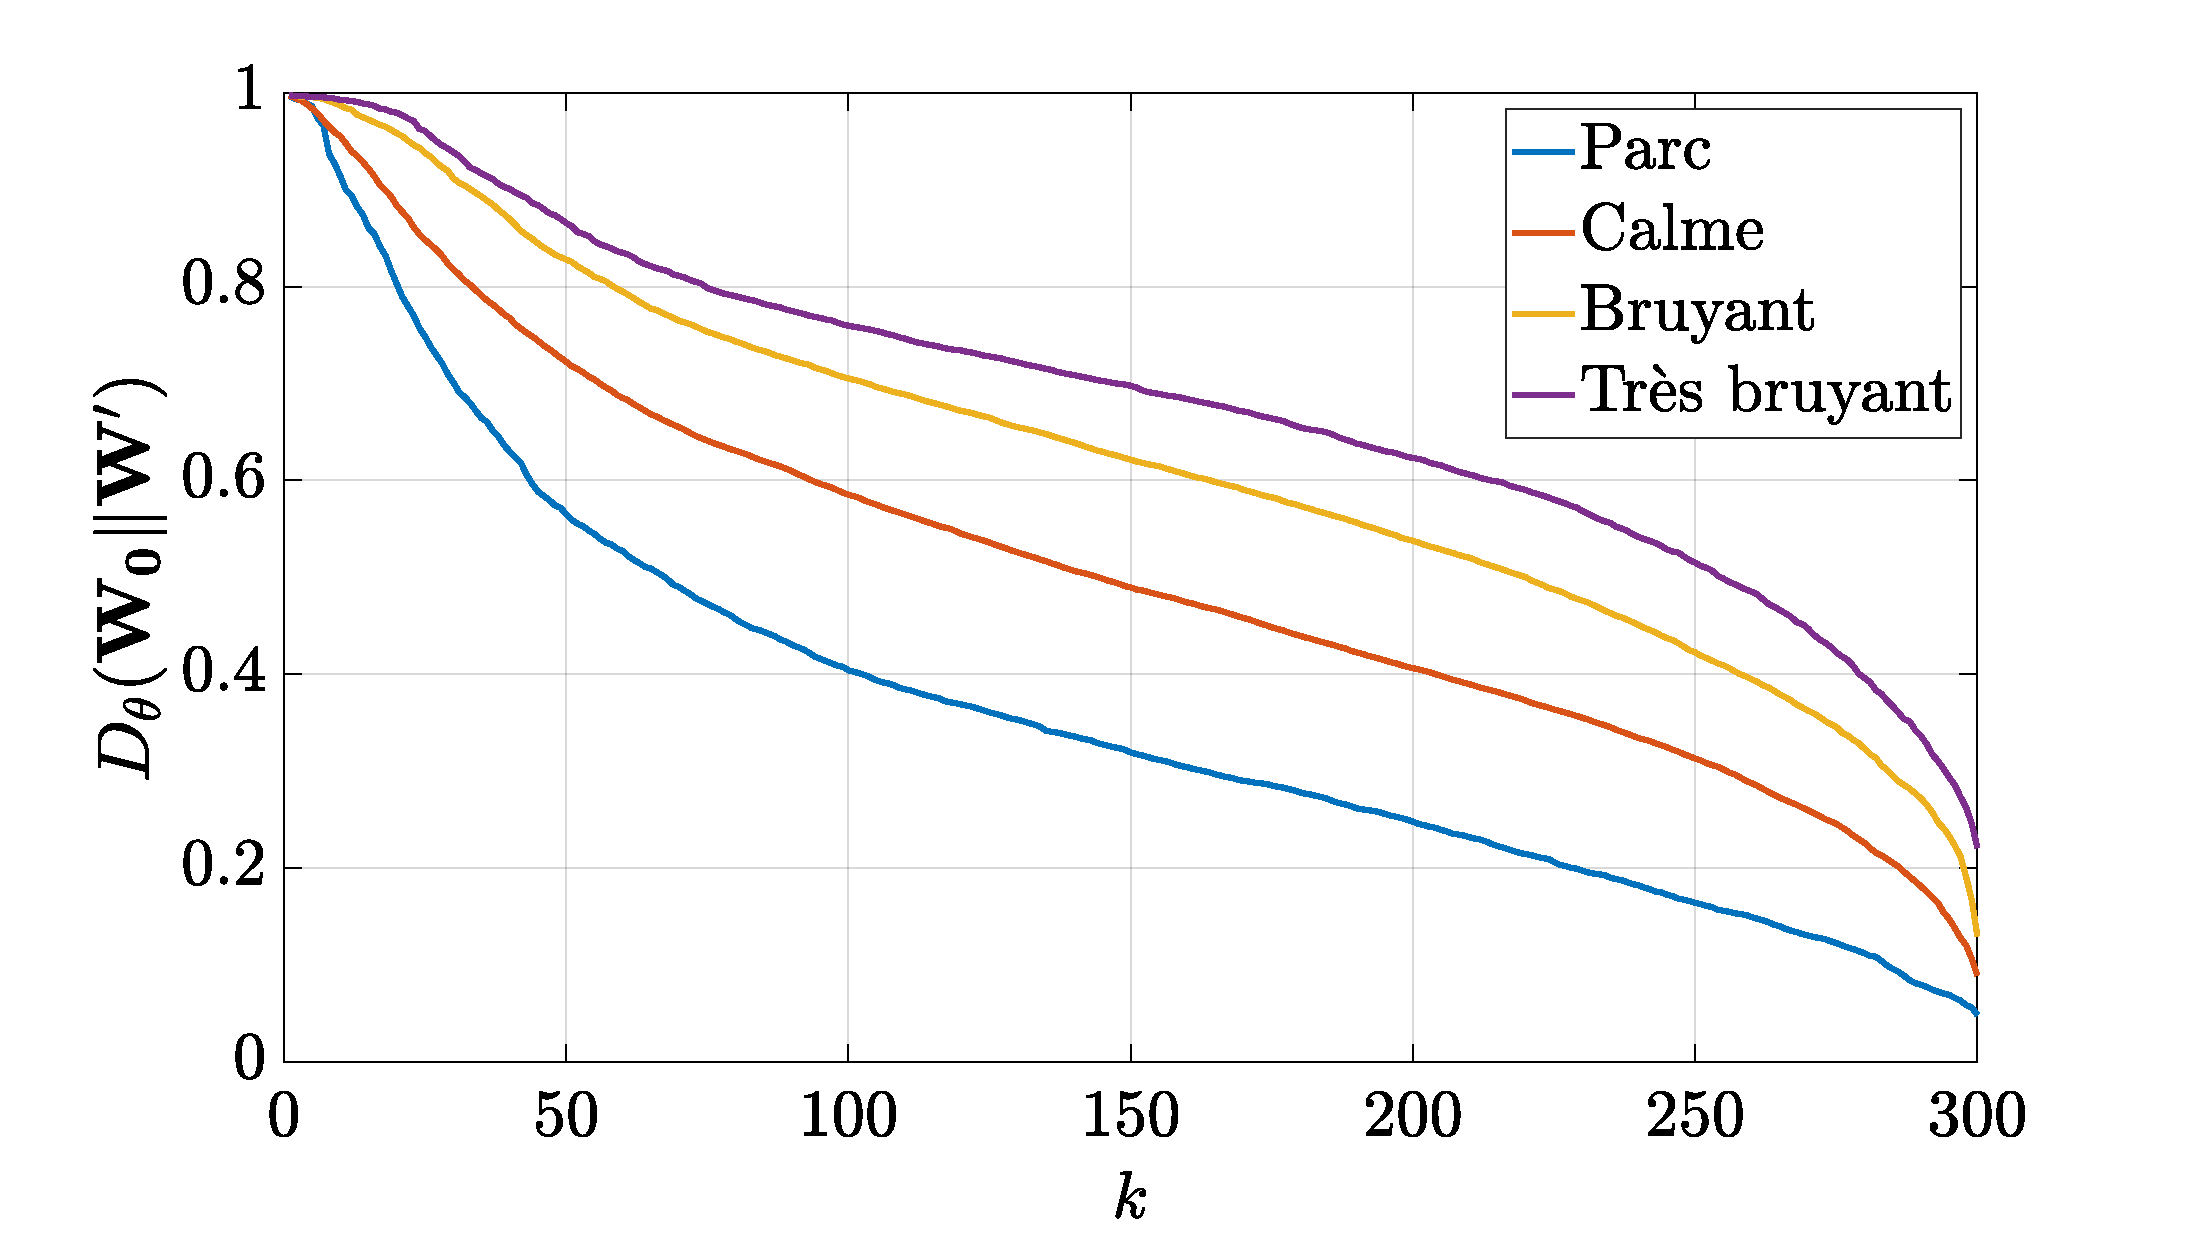
\includegraphics[width=.7\linewidth]{./figures/resultats/dist_grafic.pdf}
\caption{Distances $D(\mathbf{W_0}\Vert \mathbf{W'})$ moyennes par ambiance sonore triées par ordre décroissant.}
\label{fig:dist_grafic}
\end{figure}

L'erreur par ambiance sonore est ensuite détaillée selon les combinaisons optimales de chaque méthode. Le temps de calcul mis par l'estimateur pour extraire la composante \textit{trafic} d'un spectrogramme $\mathbf{V}$ d'uen durée de 1 minute est ajouté. Dans le cas de la NMF, c'est le temps mis par la méthode pour réaliser les 400 itérations.

\begin{table}[h]
\centering
\caption{Erreurs $MAE_{60}$ selon les estimateurs NMF pour chaque méthode dans sa combinaison optimale de modalités avec les estimateurs \textit{baseline} à 500 Hz et 20 kHz.}
\label{tab:erreur_mae60_amb}
\resizebox{\textwidth}{!}{%
\begin{tabular}{L{4cm}C{2.5cm}C{2.5cm}C{2.5cm}C{2.5cm}C{2.5cm}}
\toprule
méthode & Parc & Rue Calme & Rue Bruyante & Rue très bruyante & temps de calcul/min (s)\\ \midrule
filtre PB, $f_c$ = 20 kHz & 9,97 ($\pm$ 5,08) & 3,54 ($\pm$ 2,25) & 1,08 ($\pm$ 0,53)& 0,45 ($\pm$ 0,38)&  0,03 ($\pm$ 0,01) \\
filtre PB, $f_c$ = 500 Hz & 4,80 ($\pm$ 5,08) & 1,87 ($\pm$ 2,25) & 0,92 ($\pm$ 0,54) & 0,96 ($\pm$ 0,38) &  0,03 ($\pm$ 0,01) \\ \midrule
NMF SUP & 5,58 ($\pm$ 5,06)  & 2,00 ($\pm$ 2,22) & 0,66 ($\pm$ 0,56) & 0,64 ($\pm$ 0,33) & 0,19 ($\pm$ 0,03)\\
NMF SEM & 2,69 ($\pm$ 2,71) & 2,36 ($\pm$ 2,42) & 1,58 ($\pm$ 0,87) & 1,38 ($\pm$ 0,60) & 3,55 ($\pm$ 0,13)\\
NMF IS & \textbf{\textcolor{red}{2,21 ($\pm$ 3,84)}} & \textbf{\textcolor{red}{1,64 ($\pm$ 1,85)}} & \textbf{\textcolor{red}{0,61 ($\pm$ 0,54)}} &  \textbf{\textcolor{red}{0,34 ($\pm$ 0,20)}} & 4,30 ($\pm$ 0,31)\\ \bottomrule
\end{tabular}}
\end{table}

La NMF IS se révèle la méthode la plus performante pour 3 ambiances sonores. La NMF SEM propose la plus faible erreur pour les ambiances \textit{Parc} qui correspondent aux scènes où le trafic est le moins présent. 
La NMF SUP conserve son comportement : peu efficace pour les scènes sans trafic et meilleure lorsque le trafic devient prédominant. Seulement ici, la NMF IS est meilleure !

On trace l'évolution de l'erreur $MAE_{60}$ selon le nombre d'éléments dans $\mathbf{W}$ pour la NMF IS dans sa combinaison optimale. On étend pour ce cas la dimension du dictionnaire jusqu'à 400 éléments. En parallèle de cette évolution le temps de calcul est adjoint. Il permet de constater l'influence du nombre d'éléments dans la NMF IS : l'erreur décroit avec l'augmentation de $\mathbf{K}$. Plus d'éléments dans le dictionnaire implique d'avoir plus de spectre et ainsi de mieux modéliser les variations de la source sonore. Cependant, cette diminution se fait au dépend du temps de calcul : celui-ci croit avec l'augmentation du rang du dictionnaire. Si entre $K$ = 25 et $K$ = 200, l'erreur chute significativement, à partir de $K$= 300 la diminution de l'erreur devient faible, la variation de l'erreur devient faible au regard de la variation du temps de calcul. Suivant les applications souhaités, il peut ne pas être judicieux d'augmenter la taille du dictionnaire.

\begin{figure}[h]
\centering
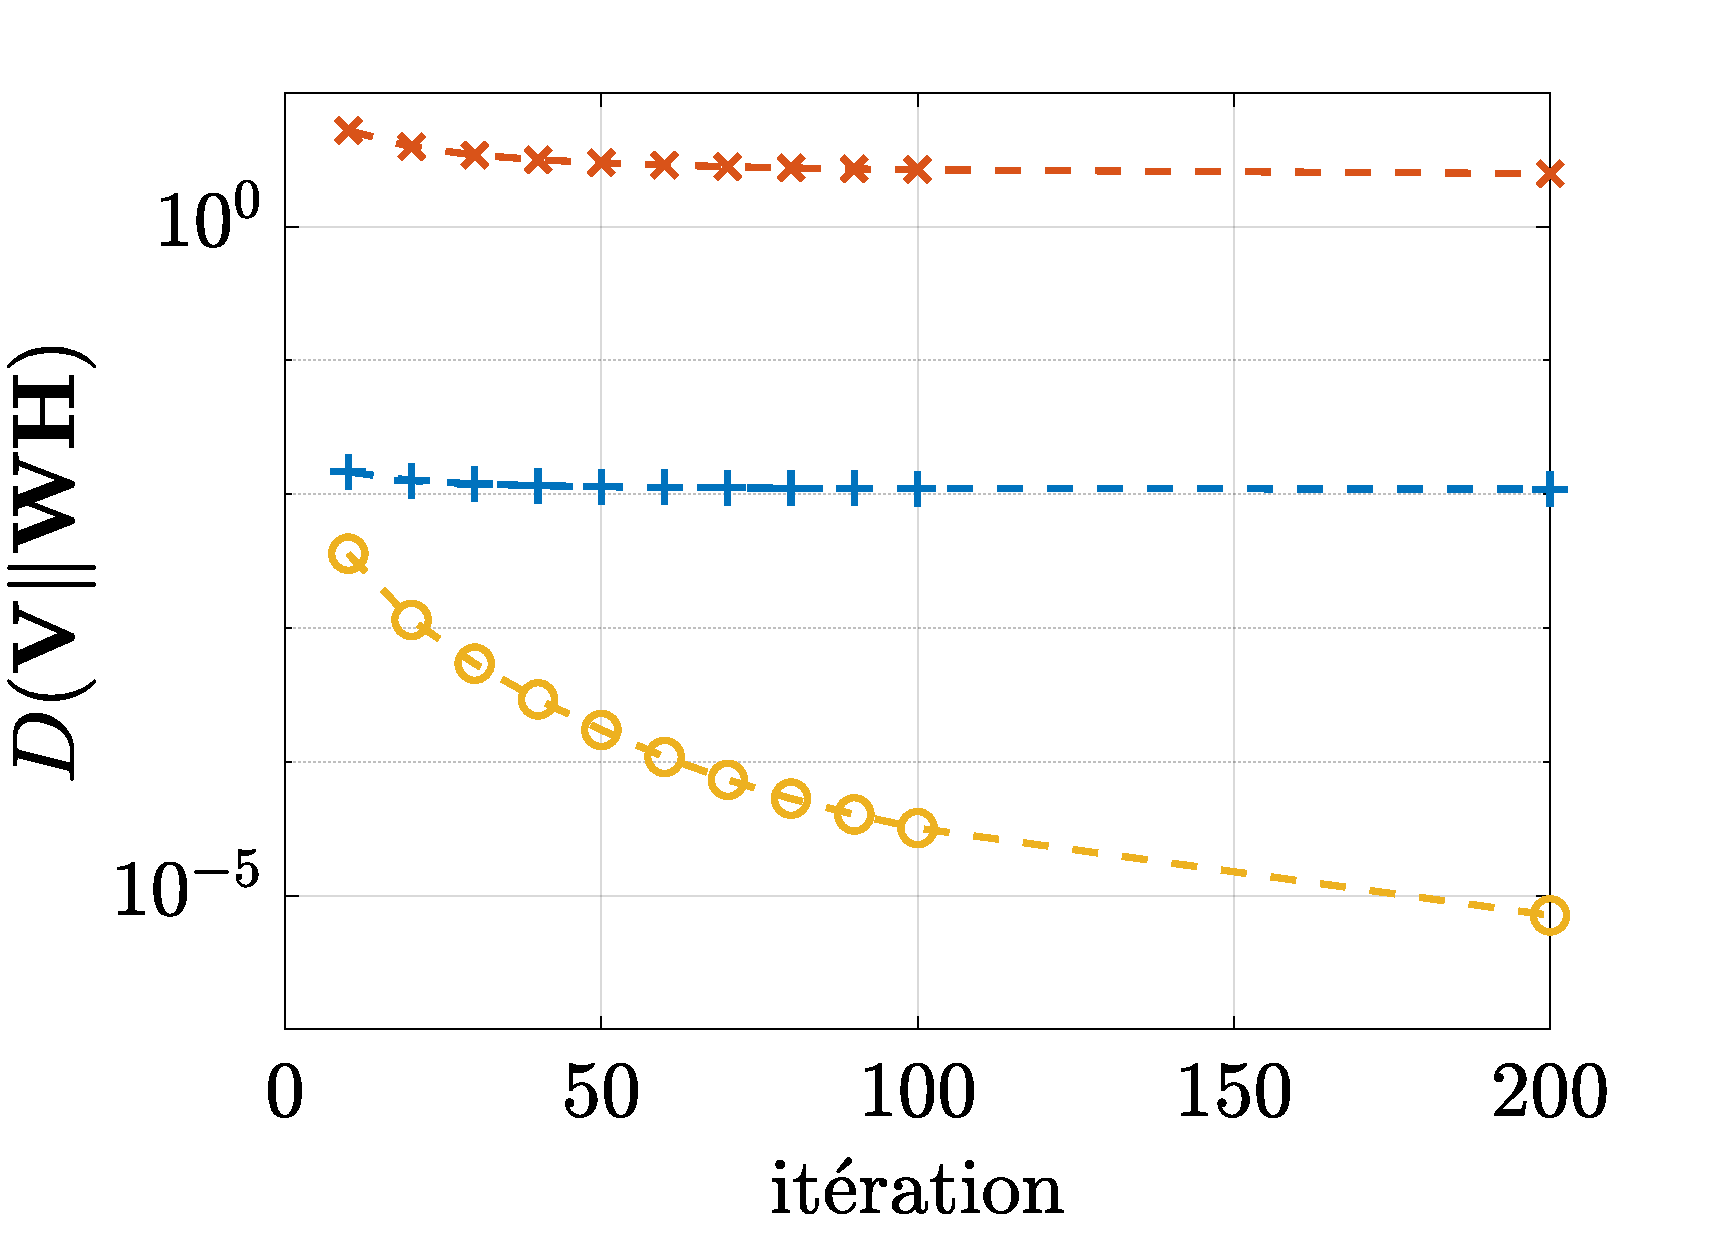
\includegraphics[width=.8\linewidth]{./figures/resultats/grafic_cost.pdf}
\caption{Fonction de coût moyen pour le corpus élémentaire SOUR selon les 3 NMF pour leur combinaison de facteurs optimale}
\end{figure}


La convergence de la NMF IS est meilleure sur l'ensemble des cas, la SEM est la moins efficace y compris sur l'ambiance \textit{parc} alors qu'elle y obtient la plus faible erreur. La NMF SUP et SEM sont rapidement constante, la mise à jour des matrices ne permettent pas d'améliorer la reconstruction de $\mathbf{V}$, la NMF IS, en mettant à jour $\mathbf{W}$ et $\mathbf{H}$ permet d'améliorer progressivement la reconstruction. En définitive, améliorant la reconstruction globale, elle arrive à en obtenir une meilleure du signal \textit{trafic}.



\begin{itemize}
\item résultats
\begin{itemize}
\item allure des courbes Lp,1s pour chaque ambiance

\item smoothness VVV et impact notable sur le semi-supervisée
\item optimisation de la valeur seuil en fonction d'indicateur
calibration qui fait défaut donc les valeurs de référence sont à revoir mais ça signifie qu'avec des indicateurs assez simple, on peut ajuster les seuils et optimiser tout cela !.
\end{itemize}
\end{itemize}


\section{Pistes d'amélioration}

Plusieurs pistes sont à envisager pour améliorer l'estimation du niveau sonore du trafic. L'une des première est l'application de la contrainte de régularité temporelle sur les activateurs.

\subsection{Contrainte de régularité temporelle}
Afin de tenter d'améliorer ces résultats, une première contrainte est ajoutée sur la NMF par la contrainte de régularité temporelle. 

\begin{equation}
D(\mathbf{V}\Vert \mathbf{WH}) + \alpha C(H)
\end{equation}

Cette contrainte, présentée dans la partie \ref{} consiste à forcer les activateurs temporelles à adopter des variations plus lentes entre les trames temporelles. Son utilisation est justifié ici par le comportement de la source d'intérêt : le passage d'une voiture est un évènement qui a une durée de plusieurs secondes. En forçant les activateurs à adopter des variations plus lentes, on serait à même de pouvoir mieux modéliser cette source. 

Dans les cas de la NMF SUP et le NMF IS, cette contrainte s'applique sur l'ensemble des matrices $\mathbf{H}$. Dans le cas de la NMF SEM, le dictionnaire se décompose en deux parties (une partie fixe $\mathbf{W_s}$ composée de spectres \textit{trafic} et d'une partie mobile $\mathbf{W_r}$). Pour favoriser les variations lentes des activateurs temporelles des spectres \textit{trafic}, cette contrainte est donc seulement posée pour $\mathbf{H_s}$. La mise à jour de la matrice suit donc celle de l'équation \ref{eq:HupdateSmooth}. La mise à jour de $\mathbf{H_r}$ reste la même (équation \ref{eq:HupdateMM}).
Les valeurs de la pondération $\alpha$ permettent alors de contrôler l'influence de la contrainte. Elle est définit pour plusieurs valeurs : $\alpha = \lbrace 0,01,~ 0,05,~ 0,1,~ 0,5,~ 1,~2 \rbrace$.

L'impact de la contrainte sur la distance $D(\mathbf{V}\Vert \mathbf{WH})$ peut s'observer sur la fonction de coût. En raison de l'ajout d'un second terme, la fonction de coût est naturellement plus élevée. Sa valeur étant plus élevée, la reconstruction du signal global, après 400 itérations, est donc moins bonne que sans la pondération.
 
\begin{figure}[h]
\centering
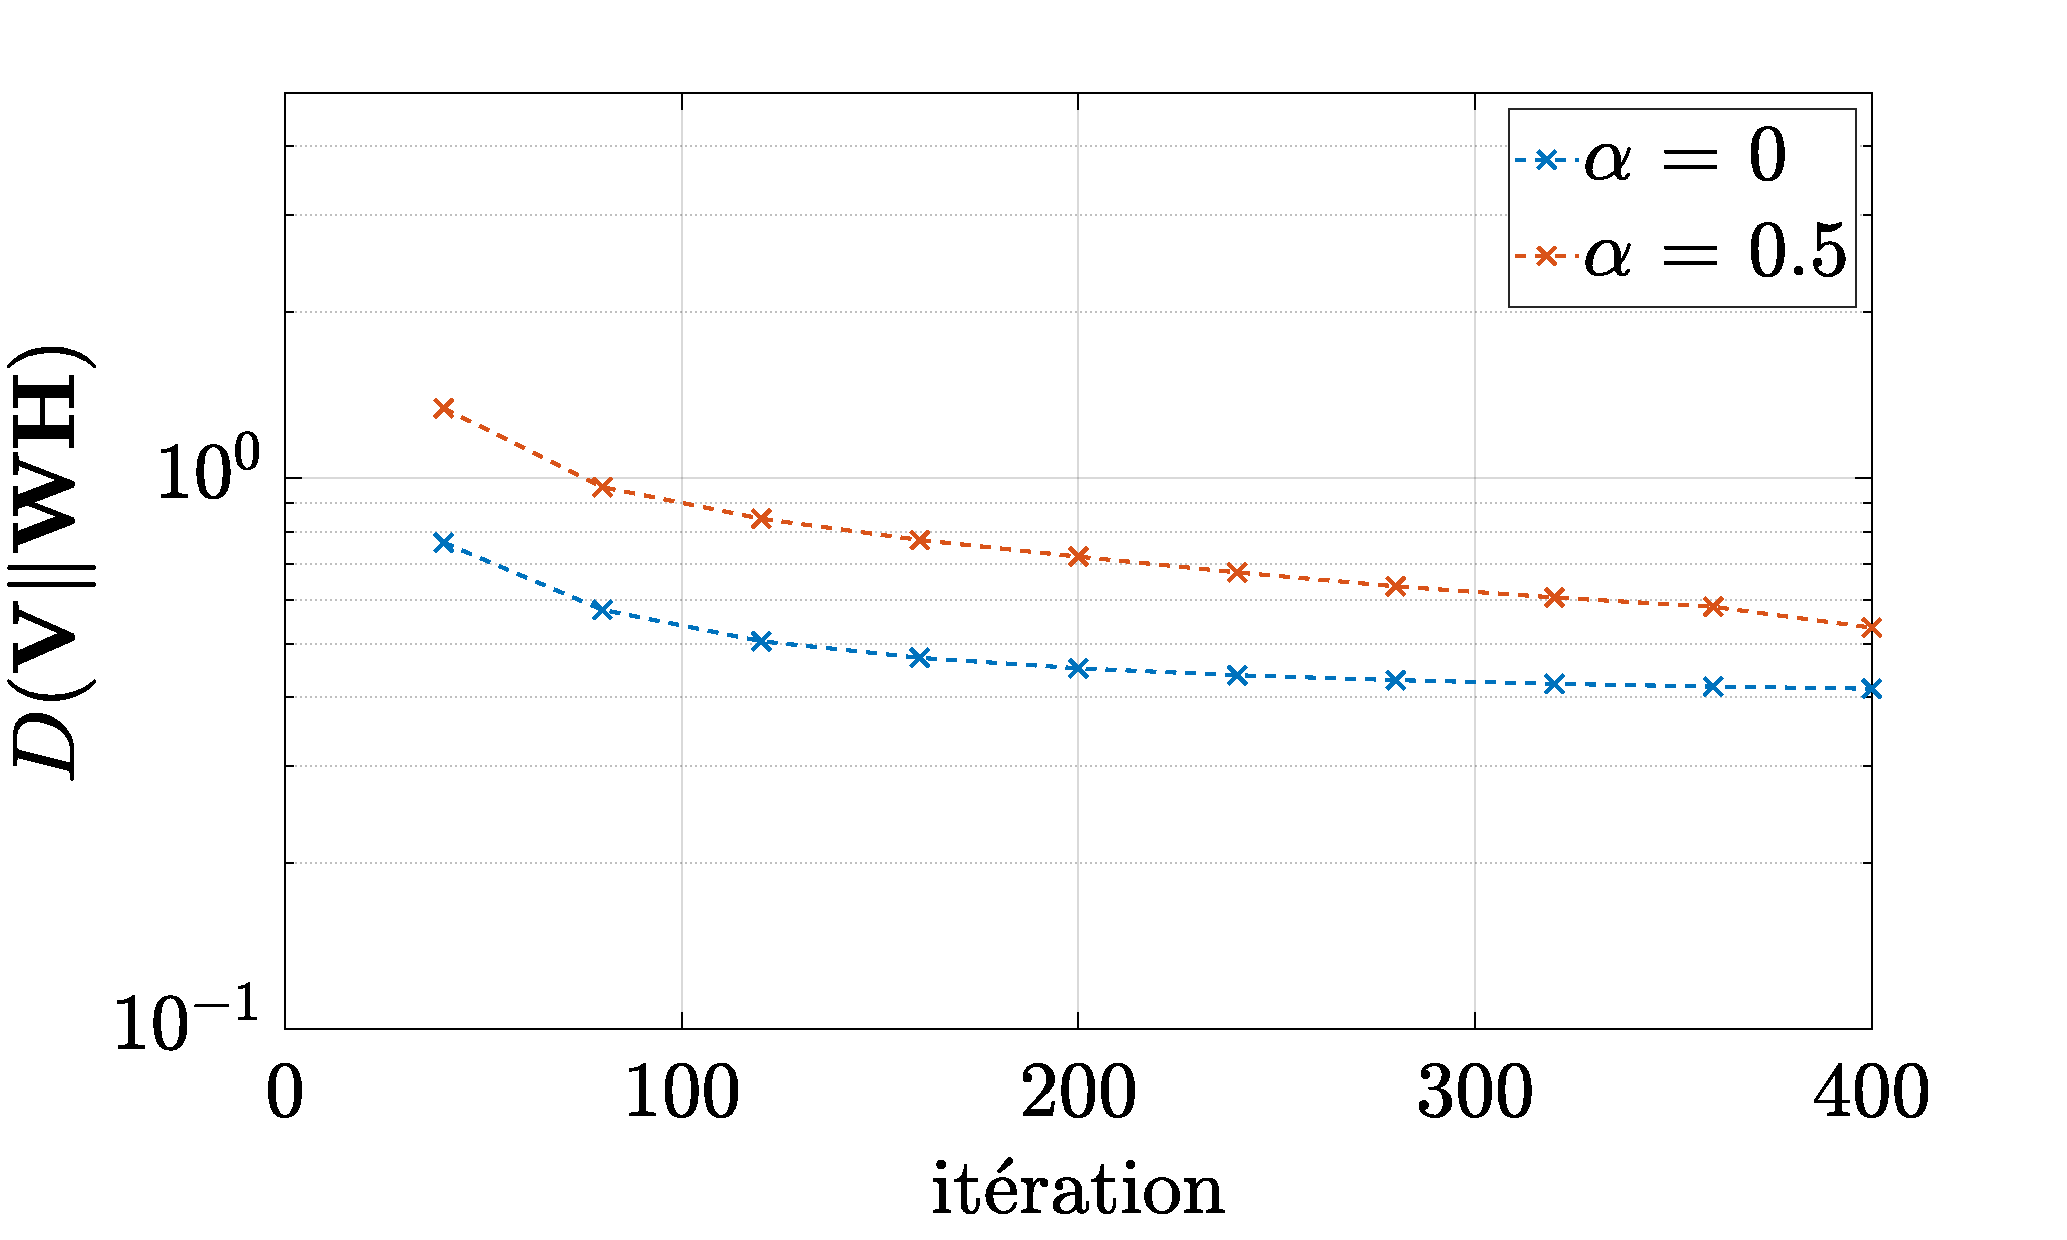
\includegraphics[width=.8\linewidth]{./figures/resultats/grafic_smooth_cost_beta0.pdf}
\caption{Influence de la régularité temporelle sur la fonction de coût pour $\beta$ = , $w_t$ = et $K$ = .}
\end{figure}

Toutefois, la reconstruction global du signal n'est pas nécessairement signe que celle de la composante \textit{trafic} soit moins bonne. On résume dans le Tableau \ref{tab:erreur_smooth}, les erreurs minimales obtenues avec la NMF SUP, SEM et IS sans pondératon et avec pondération. On ajoute lorsque la combinaison optimale de modalités avec pondération diffère de celle sans pondération, son erreur afin de pouvoir évaluer son effet.

\begin{table}[h]
\centering
\caption{Erreurs $MAE_{60}$ pour chaque estimateur NMF avec la contrainte de régularité $\alpha$.}
\label{tab:erreur_smooth}
\begin{tabular}{L{2cm}C{1.2cm}C{1.2cm}C{1.2cm}C{1.2cm}C{1.2cm}C{2.5cm}}
\toprule
 & $\beta$ & $K$ & $w_t$ & $t_h$ & $\alpha$ & $MAE_{60}$ \\ \midrule
\multirow{2}{*}{NMF SUP} & 2 & 25 & 0,5 & - & 0 & 2,22 ($\pm$ 2,33) \\
 & 2 & 25 & 0,5 & - & 0,01 & \textbf{2,13 ($\pm$ 2,20)} \\\midrule
\multirow{3}{*}{NMF SEM} & 1 & 300 & 2 & - & 0 & 1,98 ($\pm$ 0,51) \\
 & 1 & 300 & 2 & - & 0,10 & 1,87 ($\pm$ 0,41) \\
 & 0 & 300 & 2 & - & 0,50 & \textbf{1,55 ($\pm$ 0,98)} \\\midrule
\multicolumn{1}{c}{\multirow{2}{*}{NMF IS}} & \textbf{2} & \textbf{300} & \textbf{1} & \textbf{0,35} & \textbf{0} & \textbf{\textcolor{red}{1,20 ($\pm$ 0,87)}} \\
\multicolumn{1}{c}{} & 1 & 200 & 1 & 0,36 & 0,15 & 1,47 ($\pm$ 0,86)\\ \bottomrule
\end{tabular}
\end{table}

Pas d'effet de la contrainte de smoothness sur la NMF IS, par contre effet pour la NMF SEM. Si l'effet est peu important pour la même combinaison de modalité, la NMF SEM avec $\beta$ = 0 offre une plus faible erreur notable. L'erreur $MAE_{60}$ par ambiance sonore est tracé pour ces trois méthodes afin de voir son impact.



Dans la Figure, on compare la méthode optimale sans pondération, la combinaison pour $\beta$ = 0 sans et avec pondération. L'impact de la pondération pour le cas $\beta$ = 0 est significatif. Pour le cas sans pondération, l'erreur est principalement important pour les ambiances \textit{Calme} et \textit{Bruyant}. Avec la contrainte de régularité, cette distribution évolue et évolution de façon similaire au $\beta$ = 1 : une erreur plus importante pour l'ambiance \textit{Parc} pour progressivement diminuer au fur et à mesure que le trafic devient prédominant.
En conclusion, un système totalement libre, si il permet, de prime abord plus de possibilité, doit ici être contraint afin que cette liberté soit limitée. 

\begin{figure}[h!]
\centering
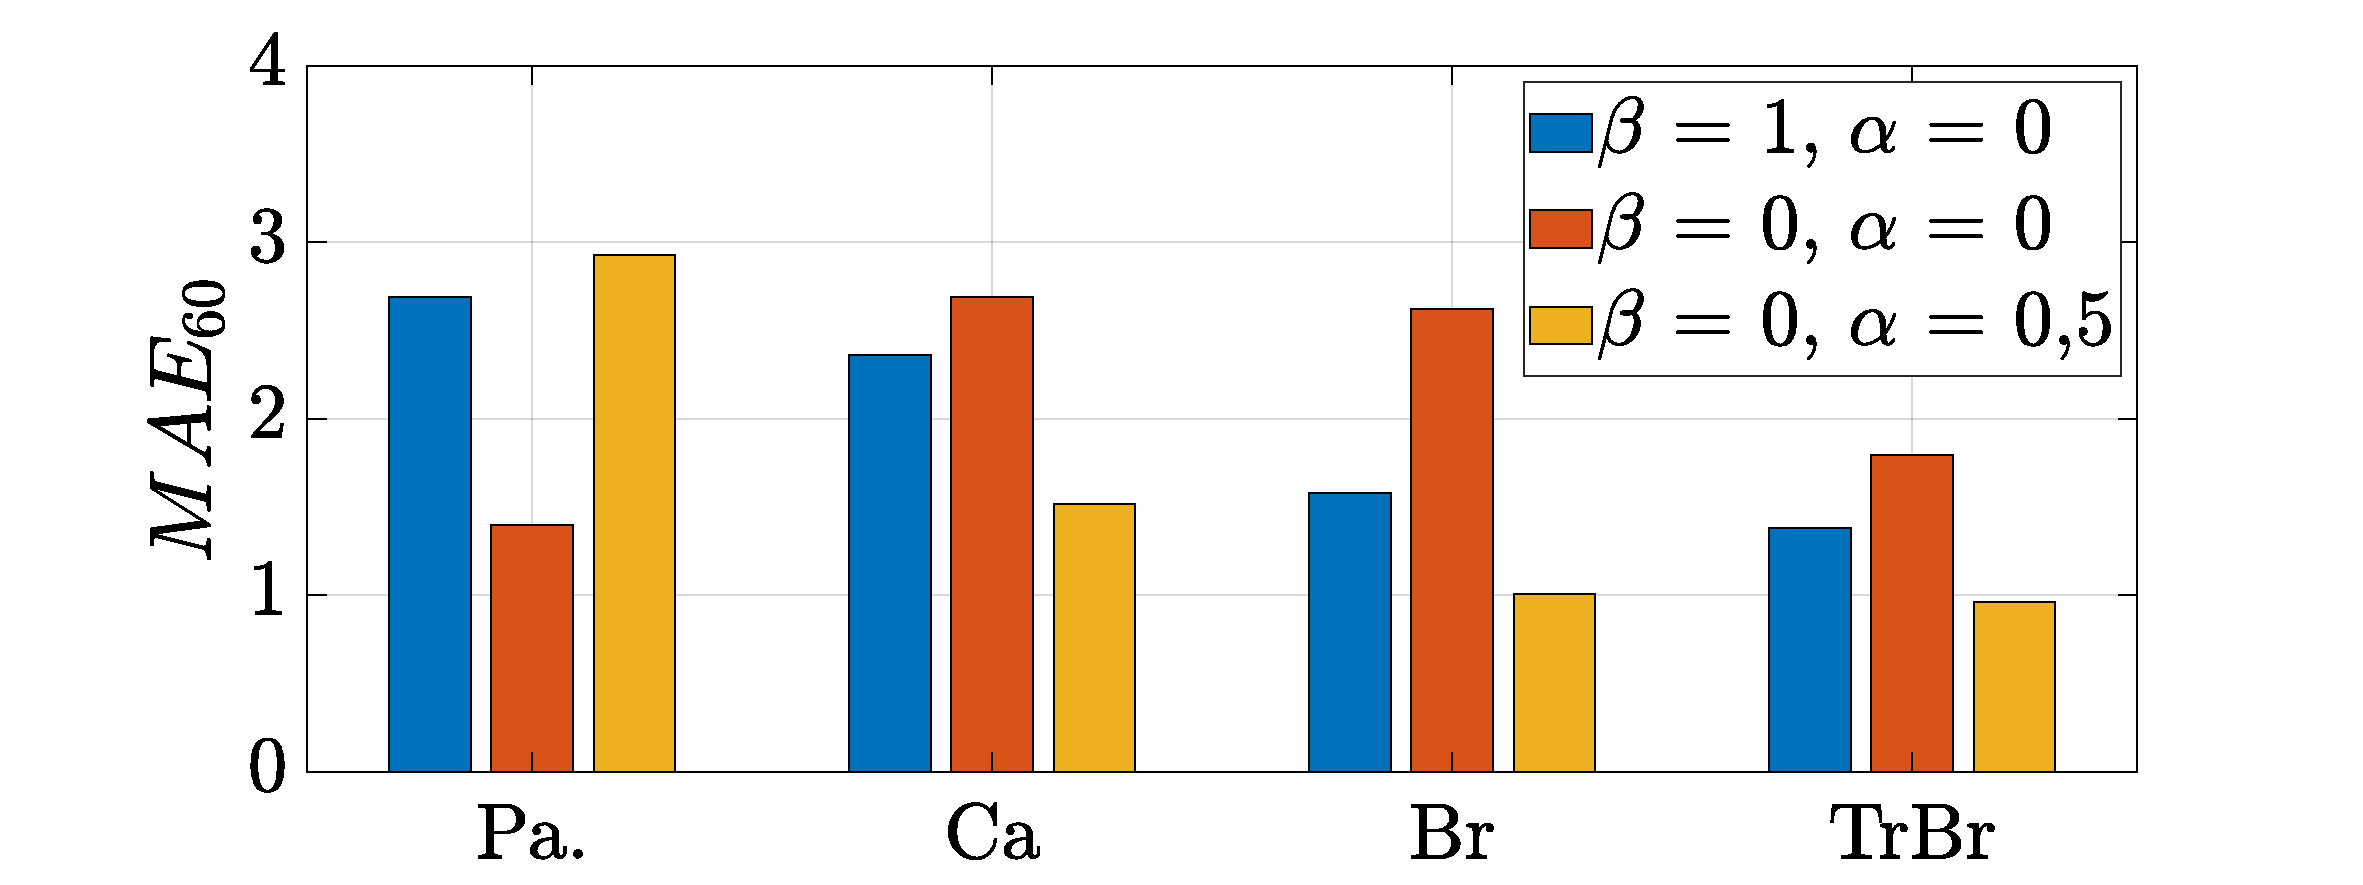
\includegraphics[width=.9\linewidth]{./figures/resultats/grafic_smooth_bar.pdf}
\caption{Influence de la pondération de régularité temporelle pour la NMF SEM selon chaque ambiance sonore.}
\end{figure}




\subsection{Contrainte par parcimonie}



\subsection{Optimisation par les seuils}


%On a déterminé un seuil optimal par ambiance :
%parc => th = 
%calme => th = 
%br => th = 
%tr_br=> th = 

Le but est de trouver des indicateurs simples qui serait corrélé à ces seuils


%\end{document}